\section{Date: 2026-09-26}
\noindent \textbf{Series ID: A261RE1A156NBEA} 

\noindent This series is titled Shares of gross domestic income and has a frequency of Annual. The units are Percent and the seasonal adjustment is Not Seasonally Adjusted.The observation start date is 1929-01-01 and the observation end date is 2024-01-01.The popularity of this series is 3. \\ 

\noindent \textbf{Series ID: ATNHPIUS37764Q} 

\noindent This series is titled All-Transactions House Price Index for Peabody, MA (MSAD) (DISCONTINUED) and has a frequency of Quarterly. The units are Index 1995:Q1=100 and the seasonal adjustment is Not Seasonally Adjusted.The observation start date is 1979-07-01 and the observation end date is 2013-01-01.The popularity of this series is 1. \\ 

\subsection{Raw Regression}
\noindent Regresses the two series against each other directly. A significant result here can come just as easily from both series sharing a long-run trend as from any real relationship.

\begin{center}
\begin{tabular}{lclc}
\toprule
\textbf{Dep. Variable:}               & value\_fred\_ATNHPIUS37764Q & \textbf{  R-squared:         } &    -0.000   \\
\textbf{Model:}                       &             OLS             & \textbf{  Adj. R-squared:    } &    -0.000   \\
\textbf{Method:}                      &        Least Squares        & \textbf{  F-statistic:       } &       nan   \\
\textbf{Date:}                        &       Sat, 26 Sep 2026      & \textbf{  Prob (F-statistic):} &      nan    \\
\textbf{Time:}                        &           15:12:54          & \textbf{  Log-Likelihood:    } &   -191.64   \\
\textbf{No. Observations:}            &                34           & \textbf{  AIC:               } &     385.3   \\
\textbf{Df Residuals:}                &                33           & \textbf{  BIC:               } &     386.8   \\
\textbf{Df Model:}                    &                 0           & \textbf{                     } &             \\
\textbf{Covariance Type:}             &          nonrobust          & \textbf{                     } &             \\
\bottomrule
\end{tabular}
\begin{tabular}{lcccccc}
                                      & \textbf{coef} & \textbf{std err} & \textbf{t} & \textbf{P$> |$t$|$} & \textbf{[0.025} & \textbf{0.975]}  \\
\midrule
\textbf{value\_fred\_A261RE1A156NBEA} &       1.4129  &        0.118     &    11.962  &         0.000        &        1.173    &        1.653     \\
\bottomrule
\end{tabular}
\begin{tabular}{lclc}
\textbf{Omnibus:}       &  8.793 & \textbf{  Durbin-Watson:     } &    0.027  \\
\textbf{Prob(Omnibus):} &  0.012 & \textbf{  Jarque-Bera (JB):  } &    2.581  \\
\textbf{Skew:}          &  0.231 & \textbf{  Prob(JB):          } &    0.275  \\
\textbf{Kurtosis:}      &  1.732 & \textbf{  Cond. No.          } &     1.00  \\
\bottomrule
\end{tabular}
%\caption{OLS Regression Results}
\end{center}

Notes: \newline
 [1] Standard Errors assume that the covariance matrix of the errors is correctly specified.

\begin{figure}
\centering
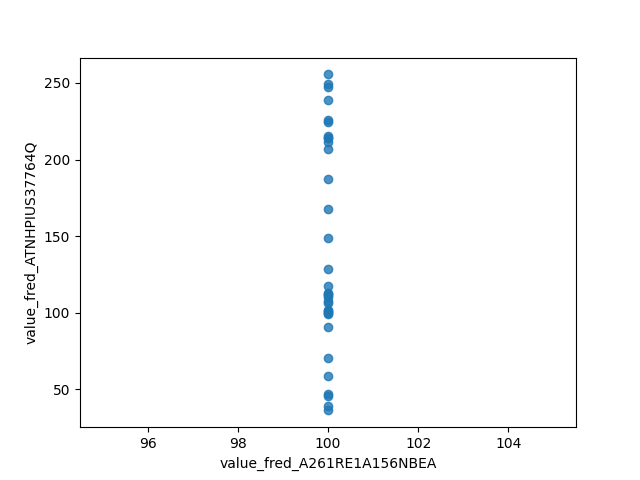
\includegraphics[scale = 0.9]{plots/plot_2026-09-26.png}
\caption{Raw Regression Plot for 2026-09-26}
\end{figure}
\newpage
\subsection{Detrended Regression}
\noindent Regresses the residuals of each series after removing its own linear time trend, so a shared trend can no longer drive the result on its own. A relationship that stays significant here is better evidence of a genuine link between the two series.

\begin{center}
\begin{tabular}{lclc}
\toprule
\textbf{Dep. Variable:}                          & value\_fred\_ATNHPIUS37764Q\_detrended & \textbf{  R-squared:         } &     0.002   \\
\textbf{Model:}                                  &                  OLS                   & \textbf{  Adj. R-squared:    } &    -0.030   \\
\textbf{Method:}                                 &             Least Squares              & \textbf{  F-statistic:       } &   0.04974   \\
\textbf{Date:}                                   &            Sat, 26 Sep 2026            & \textbf{  Prob (F-statistic):} &    0.825    \\
\textbf{Time:}                                   &                15:12:54                & \textbf{  Log-Likelihood:    } &   -157.44   \\
\textbf{No. Observations:}                       &                     34                 & \textbf{  AIC:               } &     318.9   \\
\textbf{Df Residuals:}                           &                     32                 & \textbf{  BIC:               } &     321.9   \\
\textbf{Df Model:}                               &                      1                 & \textbf{                     } &             \\
\textbf{Covariance Type:}                        &               nonrobust                & \textbf{                     } &             \\
\bottomrule
\end{tabular}
\begin{tabular}{lcccccc}
                                                 & \textbf{coef} & \textbf{std err} & \textbf{t} & \textbf{P$> |$t$|$} & \textbf{[0.025} & \textbf{0.975]}  \\
\midrule
\textbf{const}                                   &     -29.7625  &      133.528     &    -0.223  &         0.825        &     -301.750    &      242.225     \\
\textbf{value\_fred\_A261RE1A156NBEA\_detrended} &     5.71e+13  &     2.56e+14     &     0.223  &         0.825        &    -4.64e+14    &     5.79e+14     \\
\bottomrule
\end{tabular}
\begin{tabular}{lclc}
\textbf{Omnibus:}       &  2.062 & \textbf{  Durbin-Watson:     } &    0.159  \\
\textbf{Prob(Omnibus):} &  0.357 & \textbf{  Jarque-Bera (JB):  } &    1.548  \\
\textbf{Skew:}          &  0.330 & \textbf{  Prob(JB):          } &    0.461  \\
\textbf{Kurtosis:}      &  2.190 & \textbf{  Cond. No.          } & 5.84e+13  \\
\bottomrule
\end{tabular}
%\caption{OLS Regression Results}
\end{center}

Notes: \newline
 [1] Standard Errors assume that the covariance matrix of the errors is correctly specified. \newline
 [2] The smallest eigenvalue is 9.98e-27. This might indicate that there are \newline
 strong multicollinearity problems or that the design matrix is singular.

\begin{figure}
\centering
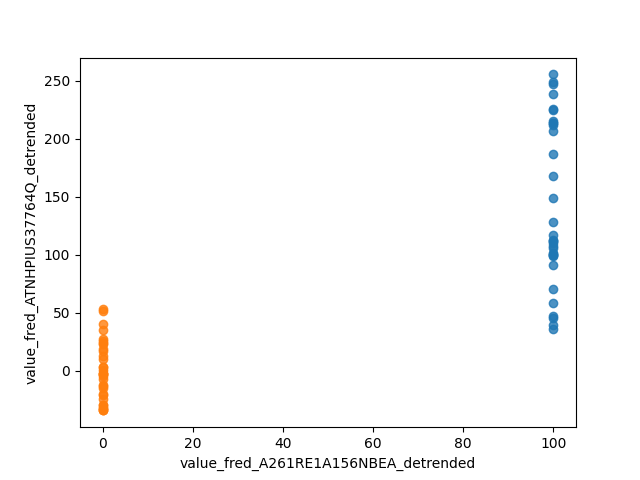
\includegraphics[scale = 0.9]{plots/plot_2026-09-26_detrended.png}
\caption{Detrended Regression Plot for 2026-09-26}
\end{figure}
\newpage
